\documentclass{exam}
\usepackage[utf8]{inputenc}

\usepackage[parfill]{parskip}
\usepackage[dvipsnames]{xcolor}
\usepackage{amsmath}
\usepackage{amsfonts}
\usepackage{amsthm}
\usepackage{microtype}
\usepackage{siunitx}
\DeclareSIUnit\year{yr}
\usepackage{pgfplots}
\usepackage{graphicx}
\usepackage{sidecap}
\sidecaptionvpos{figure}{c}
\usepackage{float}
\usepackage{gensymb}
\usepackage{tkz-euclide}
\usetkzobj{all}
\usepackage{commath}
\usepackage{hyperref}
\usepackage{enumitem}
\usepackage{wasysym}
\usepackage{tabularx}

\renewcommand*{\thefootnote}{\fnsymbol{footnote}}

\newtheorem*{thm}{Theorem}
\newtheorem*{iden}{Identity}
\newtheorem*{lemma}{Lemma}
\theoremstyle{definition}
\newtheorem*{defn}{Definition}
\newtheorem*{ex}{Example}

% russian integral
\usepackage{scalerel}
\DeclareMathOperator*{\rint}{\scalerel*{\rotatebox{17}{$\!\int\!$}}{\int}}

\pgfplotsset{vasymptote/.style={
    before end axis/.append code={
        \draw[densely dashed] ({rel axis cs:0,0} -| {axis cs:#1,0})
        -- ({rel axis cs:0,1} -| {axis cs:#1,0});
    }
}}

% \qformat{Question \thequestion: \thequestiontitle\hfill}

\begin{document}

\section*{NCEA Level 3 Calculus\\Exam Advice}

Now is the time when I pass on my exam-taking wisdom in bullet-point list form.

\begin{itemize}
  \item Don't cram the night before the exam. Get a good night's sleep and have a proper meal for breakfast.
  \item Prepare your exam bag the night before. Know the earthquake procedures and have an emergency pack.
  \item Stay calm and be confident.
  \item If you forget how numbers work, try counting your fingers and work upwards from there. (Quality advice from a former Scholarship candidate.)
  \item Draw a diagram if one isn't given.
  \item Don't study by reading examples, study by doing problems.
  \item Read through all the questions before attempting any of them.
  \item Have a problem-solving strategy.
  \item Begin by working out the part of the standard the question is asking about.
  \item Show all your work.
  \item Never leave a problem blank.
  \item If you're stuck, move on and do another question.
  \item Write sentences, not symbols. Use correct spelling, grammar. and punctuation??!
  \item \textbf{If the question gives you a hint, there's probably a reason for that!}
\end{itemize}

Scholarship exams especially are a competition between you and the examiner. They want to impress you with the difficulty of the
questions that they throw at you, \textbf{but you can meet that challenge.} There is nothing that they can chuck your way that cannot
be done with level three material (because they're not allowed to), and so the way to get through a scholarship question is usually
to work methodically.

Remember that mathematics is difficult, and that it took hundreds of years for humanity to discover the concepts and techniques
which you will apply in the three hours of an NZQA external examination.

\begin{center}
  
\includegraphics[height=0.2\textheight]{justdoit}
  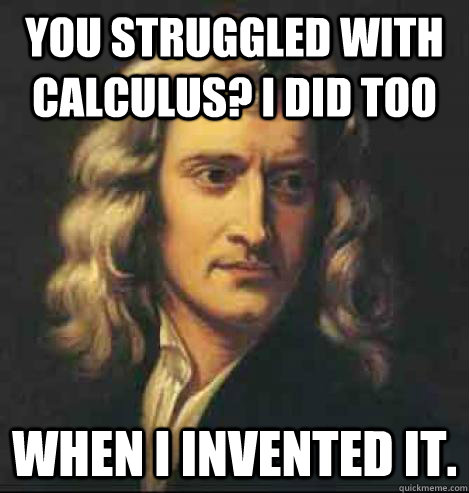
\includegraphics[height=0.2\textheight]{meme2}
\end{center}

\clearpage
\subsection*{Study Skills for Mathematics}
(From the University of Cambridge)

[Examinations are] designed to test your knowledge of the courses you have attended rather than your ability to jump through mathematical hoops. Nevertheless, strategy matters. Extreme marks (either high or low) are available in mathematics examinations, which means that playing the cards you hold to best advantage is of vital importance.

Here are some thoughts; you've heard them all before, but that does not make them any less worth saying. The examinations may besome way off, but you will find that good examination technique can be acquired over the course of the year by making suitable preparations and developing good habits. (For example, the first two points
assume that your year's work is in good order.)

\begin{itemize}
  \item For revision, work through examples while reading the relevant section of your notes (just reading is not enough).

  \item For last minute preparation, look through your supervision work to remind yourself how to do questions.

  \item In the examination, above all, stay cool --- if it is hard for you, it is probably hard for everyone.

  \item Don't rush into a question --- read the whole paper carefully and
        start with the question you feel most confident about.

  \item Analyse exactly what you are being asked to do; try to under-
        stand the hints (explicit and implicit); remember to distinguish
        between terms such as explain/prove/define/etc.

  \item Remember that different parts of a question are often linked (it
        is usually obvious from the notation and choice of variables).\footnote{~This is
        less relevant for modern NCEA examinations (even the last 2-3 Scholarship exams).}

  \item Set out your answer legibly and logically (don't scribble down
        the first thought that comes into your head) --- this not only
        helps you to avoid silly mistakes but also signals to the examiner
        that you know what you are doing (which can be effective even
        if you haven't the foggiest idea what you are doing).

  \item If you get stuck, state in words what you are trying to do and
        move on (at E-level, you don't get credit for merely stating
        intentions, but university examiners are generally grateful for
        any sign of intelligent life).
\end{itemize}

\end{document}
